\documentclass[a4paper, 11pt]{article}
\usepackage[utf8]{inputenc}
\usepackage{pgffor}
\usepackage{ifthen}
\usepackage{amsmath}
\usepackage{amssymb}
\usepackage[swedish]{babel}
\usepackage[arrowdel]{physics}
\usepackage{graphicx}

\newcommand{\proof}{\subparagraph{Bevis}}
\newcommand{\vect}[1]{\vectorbold{#1}}
\newcommand{\bound}[1]{\partial #1}
\newcommand{\limit}[2]{\lim\limits_{#1\to #2}}
\newcommand{\deval}[4][]{\dv[#1]{#2}{#3} (#4)}
\newcommand{\pdeval}[4][]{\pdv[#1]{#2}{#3} (#4)}
\newcommand{\inteval}[3]
{
	\int\limits_{#1}{#2}(#3)
	\foreach \variable in #3
	{
		\ifthenelse{\equal{\variable}{\dots}}
			{}
			{\dd{\variable}}
	}
}
\newcommand{\cint}[4][o]
{
	\ifthenelse{\equal{#1}{c}}
		{\oint}
		{\int}
	\limits_{#2} #3\cdot\dd{#4}
}
\newcommand{\fint}[3]
{
	\iint\limits_{#1} #2\cdot\dd{#3}
}

\newcommand{\N}{\mathbb{N}}
\newcommand{\Z}{\mathbb{Z}}
\newcommand{\Q}{\mathbb{Q}}
\newcommand{\R}{\mathbb{R}}
\newcommand{\C}{\mathbb{C}}

\title{Sammanfattning av SF1674 Flervariabelanalys}
\author{Yashar Honarmandi}
\date{\today}

\begin{document}\sloppy

\maketitle

\begin{abstract}
	Detta ær en sammanfattning av kursen SH1014 Modern fysik.
\end{abstract}

\pagenumbering{roman}
\thispagestyle{empty}

\newpage

\tableofcontents

\newpage

\pagenumbering{arabic}

\section{Vektoralgebra}

\subsection{Satser}

\paragraph{Cauchy-Schwarz' olikhet}
Låt $\vect{x},\vect{y}\in\R^n$. Då gäller att
\begin{align*}
	\abs{\vect{x}\cdot\vect{y}}\leq\abs{\vect{x}}\abs{\vect{y}}.
\end{align*}

\proof

\paragraph{Triangelolikheten}
Låt $\vect{x},\vect{y}\in\R^n$. Då gäller att
\begin{align*}
	\abs{\vect{x} + \vect{y}}\leq\abs{\vect{x}} + \abs{\vect{y}}.
\end{align*}

\proof

\paragraph{Omvända triangelolikheten}
Låt $\vect{x},\vect{y}\in\R^n$. Då gäller att
\begin{align*}
	\abs{\abs{\vect{x}} - \abs{\vect{y}}}\leq\abs{\vect{x} + \vect{y}}.
\end{align*}

\proof

\paragraph{Vektorer och förhållande mellan komponenter}
Låt $\vect{x}\in\R^n$ med komponenter $x_1, \dots, x_n$. Då gäller att
\begin{align*}
	\abs{x_i}\leq\abs{\vect{x}}\leq\sum\limits_{i = 1}^{n}\abs{x_i},\ i = 1, \dots, n.
\end{align*}

\proof

\section{Mängdlära}

\subsection{Definitioner}

\paragraph{Öppna klot}
Ett öppet klot i $\R^n$ centrerad i $\vect{a}$ med radius $r$ är
\begin{align*}
	\{\vect{x}\in\R^n:\ \abs{\vect{x} - \vect{a}}<r\}.
\end{align*}

\paragraph{Omgivningar till punkter}
$U\subset\R^n$ är en omgivning till $\vect{a}\in\R^n$ om $U$ innehåller något öppet klot med centrum $\vect{a}$.

\paragraph{Inre punkter}
Låt $M\subset\R^n$. $\vect{a}$ är en inre punkt till $M$ om det finns ett öppet klot kring $\vect{a}$ i $M$.

\paragraph{Yttre punkter}
Låt $M\subset\R^n$. $\vect{a}$ är en yttre punkt till $M$ om det finns ett öppet klot kring $\vect{a}$ i $M$:s komplement, definierad som $\R^n\setminus M$.

\paragraph{Randpunkter}
Låt $M\subset\R^n$. $\vect{a}$ är en randpunkt till $M$ om varje öppet klot kring $\vect{a}$ innehåller punkter i $M$ och $M$:s komplement.

\paragraph{Rand}
Mängden av alla randpunkter till en mängd $M$ är randen till $M$. Denna betecknas $\bound{M}$.

\paragraph{Öppna och slutna mängder}
En mängd är öppen om $\bound{M}$ är i $M$:s komplement och sluten om $\bound{M}$ är i $M$.

\paragraph{Begränsade mängder}
En mängd $M$ är begränsad om $\exists c > 0$ så att $\abs{\vect{x}} < c\forall \vect{x}\in M$.

\paragraph{Kompakta mängder}
En mängd är kompakt om den är sluten och begränsad.

\paragraph{Bågvis sammanhängande mängder}
$D$ är en bågvis sammanhängande mängd om varje par punkter $\vect{a}, \vect{b}\in D$ finns en kurva $\vect{x}(t), t\in [\alpha, \beta]$ så att $\vect{x}(t)\in D$ för alla $t$ och $\vect{x}(\alpha) = \vect{a}$ och $\vect{x}(\beta) = \vect{b}$.

\paragraph{Axelparallella rektangler}
En axelparallell rektangel i $\R^2$ är på formen
\begin{align*}
	\{(x, y)\ |\ a\leq x\leq b, c\leq y\leq d\}.
\end{align*}

\paragraph{Nollmängder}
En mängd $N\subset\R^2$ är en nollmängd om vi för alla $\varepsilon > 0$ kan täcka över $N$ med ändligt många axelparallella rektanglar med area mindre än eller lika med $\varepsilon$.

\paragraph{Kvadrerbara mängder}
En mängd $D\subset\R^2$ är kvadrerbar om $\bound{D}$ är en nollmängd.

\subsection{Satser}

\paragraph{Grafer som mängder}
Grafen av en kontinuerlig funktion $\phi: [a, b]\to\R$ är en nollmängd.

\proof

\section{Funktioner}

\subsection{Definitioner}

\paragraph{Grafen av en funktion}
Låt $f: D\to\R$ med $D\subset\R^2$. Grafen av $f$ är
\begin{align*}
	\{(x, y, z)\in\R^3: z = f(x, y)\}.
\end{align*}

\paragraph{Kurvor i $\R^p$}
En kurva i $\R^p$ är en funktion $t\to\vect{x}(t) = (x_1(t), \dots, x_p(t))$.

\paragraph{Lokala gränsvärden}
Låt $f: D\to\R^p$ med $D\subset\R^n$ och $\vect{a}$ vara en inre punkt eller randpunkt till $D$. $\limit{\vect{x}}{\vect{a}}f(\vect{x}) = \vect{b}$om det för varje $\varepsilon > 0$ finns ett $\delta > 0$ så att
\begin{align*}
	\abs{\vect{x} - \vect{a}} < \delta, \vect{x}\in D \implies\abs{f(\vect{x}) - \vect{b}} < \varepsilon.
\end{align*}

\paragraph{Gränsvärden mot oändligheten}
Låt $f: D\to\R^p$ med $D\subset\R^n$. $\limit{\abs{\vect{x}}}{\infty}f(\vect{x}) = \vect{b}$ om det för varje $\varepsilon > 0$ finns ett $\omega > 0$ så att
\begin{align*}
	\abs{\vect{x}} > \omega, \vect{x}\in D \implies\abs{f(\vect{x}) - \vect{b}} < \varepsilon.
\end{align*}

\paragraph{Kontinuitet}
Låt $f: D\to\R^p$ med $D\subset\R^n$. $f$ är kontinuerlig i $\vect{a}\in D$ om $\limit{\vect{x}}{\vect{a}}$ existerar och $\limit{\vect{x}}{\vect{a}} = f(\vect{a}$.

\paragraph{Likformig kontinuitet}
Låt $f: D\to\R^p$ med $D\subset\R^n$. $f$ är likformigt kontinuerlig på $D$ om det för varje $\varepsilon > 0$ finns ett $\delta > 0$ så att
\begin{align*}
	\abs{\vect{x} - \vect{y}} < \delta, \vect{x}, \vect{y}\in D \implies\abs{f(\vect{x}) - f(\vect{y})} < \varepsilon.
\end{align*}

\subsection{Satser}

\paragraph{Gränsvärden av funktioner och deras komponenter}
Låt $f: D\to\R^p$ med $D\subset\R^n$. $\limit{\vect{x}}{\vect{a}}f(\vect{x}) = \vect{b}$ är ekvivalent med att $\limit{\vect{x}}{\vect{a}}f_i(\vect{x}) = \vect{b}_i$, där subskriptet $i$ indikerar den $i$-te komponenten av varje vektor.

\proof
Detta följer direkt av att
\begin{align*}
	\abs{f_i(\vect{x}) - \vect{b}_i}\leq\abs{f(\vect{x}) - \vect{b}}\leq\sum\limits_{i = 1}^{p}\abs{f_i(\vect{x}) - \vect{b}_i}.
\end{align*}

\paragraph{Största och minsta värde för funktioner}
Låt $f: D\to\R^p$ med $D\subset\R^n$ och låt $D$ vara kompakt. Då antar $f$ ett största och ett minsta värde på $D$.

\proof

\paragraph{Definitionsmängd och likformig kontinuitet}
Låt $f: D\to\R^p$ med $D\subset\R^n$ och låt $D$ vara kompakt. Då är $f$ likformigt kontinuerlig på $D$.

\proof

\paragraph{Satsen om mellanliggande värden}
Låt $f: D\to\R^p$ med $D\subset\R^n$ och låt $D$ vara bågvis sammanhängande. Om $f$ antar värderna $f(\vect{a}), f(\vect{b})$ i $D$, antar $f$ också alla värden mellan $f(\vect{a})$ och $f(\vect{b})$.

\proof

\section{Derivata}

\subsection{Definitioner}

\paragraph{Partiella derivator}
Låt $f: D\to\R^p$ med $D\subset\R^n$. $f$ är partiellt deriverbar med avseende på $x_i$ i den inre punkten $\vect{a}\in D$ om gränsvärdet
\begin{align*}
	\limit{h}{0}\frac{f(\vect{a} + h\vect{e}_i) - f(\vect{a})}{h}
\end{align*}
existerar. Gränsvärdet kallas partiella derivatan av $f$ med avseende på $x_i$ i $\vect{a}$ och betecknas $\pdeval{f}{x_i}{\vect{a}}$.

\paragraph{Differentierbarhet}
Låt $f: D\to\R$ med $D\subset\R^n$. $f$ är differentierbar i $\vect{a}$ om $\exists A_1, \dots, A_n$ och en $\rho(\vect{h})$ så att
\begin{align*}
	f(\vect{a} + \vect{h}) - f(\vect{a}) = \sum\limits_{i = 1}^{n}A_ih_i + \abs{\vect{h}}\rho(\vect{h})
\end{align*}
och $\limit{\vect{h}}{\vect{0}}\rho(\vect{h}) = 0$. $f$ är differentierbar om detta är uppfylld för alla $\vect{a}\in D$.

\paragraph{$C^1$}
Låt $f: D\to\R$ med $D\subset\R^n$. $f$ är klass $C^1$ om $f$ är partiellt deriverbar och alla de partiella derivatorna är kontinuerliga i $D$.

\paragraph{$C^k$}
Låt $f: D\to\R$ med $D\subset\R^n$. $f$ är klass $C^k$ om $f$ alla partiella derivator till och med ordning $k$ existerar och är kontinuerliga i $D$.

\paragraph{Gradient}
Låt $f$ vara reellvärd och differentierbar i $\vect{x}$. Gradienten definieras som
\begin{align*}
	\grad{f} = \sum\limits_{i = 1}^{n}\pdeval{f}{x_i}{\vect{x}}\vect{e}_i.
\end{align*}

\paragraph{Riktningsderivata}
Låt $\abs{\vect{v}} = 1$. Derivatan av $f$ i punkten $\vect{a}$ i riktningen $\vect{v}$ är
\begin{align*}
	\grad_{\vect{u}}f = \limit{t}{0}\frac{f(\vect{a} + t\vect{v}) - f(\vect{a})}{t}.
\end{align*}

\paragraph{Stationära punkter}
$\vect{a}$ är en stationär punkt till $f$ om $\grad{f}(\vect{a}) = \vect{0}$.

\paragraph{Differentialer}
Låt $f:D\to\R$ med $D\subset\R^n$ öppen och låt $f$ vara differentierbar. Funktionen $\vect{h}\to\sum\pdeval{f}{x_i}{\vect{x}}h_i$ kallas differentialen av $f$ i $\vect{x}$ och betecknas $\dd{f} (\vect{x})$. Vid att skriva differentialen som en matris
\begin{align*}
	\dd{f} (\vect{x}) = \left[\pdeval{f}{x_1}{\vect{x}}\dots\pdeval{f}{x_n}{\vect{x}}\right]
\end{align*}
kan differentialet skrivas som en matrismultiplikation enligt
\begin{align*}
	\dd{f} (\vect{x})(\vect{h}) = \left[\pdeval{f}{x_1}{\vect{x}}\dots\pdeval{f}{x_n}{\vect{x}}\right]\vect{h}.
\end{align*}

\paragraph{Funktionalmatriser}
Låt $f:D\to\R^p$ med $D\subset\R^n$. $f$:s funktionalmatris definieras som
\begin{align*}
	\left[\begin{array}{ccc}
		\deval{f_1}{x_1}{\vect{x}} & \dots  & \deval{f_1}{x_n}{\vect{x}} \\
		\vdots                     & \ddots & \vdots \\
		\deval{f_p}{x_1}{\vect{x}} & \dots  & \deval{f_p}{x_n}{\vect{x}}
	\end{array}\right]
\end{align*}
och betecknas $f'(\vect{x}) = \dd{f} (\vect{x}) = \deval{(f_1\dots f_p)}{(x_1\dots x_n)}{\vect{x}}$.

\paragraph{Linjarisering}
Linjariseringen av en funktion $f$ ges av
\begin{align*}
	f(\vect{x} + \vect{h}) = f(\vect{x}) + \dd{f} (\vect{x})\vect{h}.
\end{align*}

\subsection{Satser}

\paragraph{Differentierbarhet och kontinuitet}
Låt $f$ vara differentierbar i $\vect{a}$. Då är $f$ kontinuerlig i $\vect{a}$.

\proof
Definitionen implicerar $\limit{\vect{h}}{\vect{0}}f(\vect{a} + \vect{h}) - f(\vect{a}) = 0$.

\paragraph{Differentierbarhet och partiell deriverbarhet}
Låt $f$ vara differentierbar i $\vect{a}$. Då är $f$ partiellt deriverbar med avseende på alla variabler i $\vect{a}$ och $\pdv{f}{x_i}(\vect{a}) = A_i$.

\proof
Med $\vect{h} = t\vect{e}_i$ ger definitionen av differentierbarhet
\begin{align*}
	\frac{f(\vect{a} + t\vect{e}_i) - f(\vect{a})}{t} = A_i + \frac{\abs{t}}{t}\rho(t\vect{e}_i).
\end{align*}
Gränsvärdet när $t$ går mot $0$ ger på den ena sidan definitionen av den partiella derivatan och $A_i$ på andra sidan.

\paragraph{Differentierbarhet av funktioner i $C^1$}
Varje $f\in C^1$ är differentierbar.

\proof
Låt $\vect{a}\in D$. Enligt envariabelsanalysens medelvärdesats har vi
\begin{align*}
	&f(\vect{a} + h_1\vect{e}_1) - f(\vect{a}) = \pdeval{f}{x_1}{\vect{a} + \theta _1h_1\vect{e}_1} \\
	&f(\vect{a} + h_1\vect{e}_1 + h_2\vect{e}_2) - f(\vect{a} + h_1\vect{e}_1) = \pdeval{f}{x_2}{\vect{a} + h_1\vect{e}_1 + \theta_2h_2\vect{e}_2} \\
	&\vdots \\
	&f(\vect{a} + \sum\limits_{i = 1}^{n}h_i\vect{e}_i) - f(\vect{a} + \sum\limits_{i = 1}^{n - 1}h_i\vect{e}_i) = \pdeval{f}{x_n}{\vect{a} + \sum\limits_{i = 1}^{n - 1}h_i\vect{e}_i + \theta_nh_n\vect{e}_n},
\end{align*}
där alla $\theta_i\in [0, 1]$. Eftersom de partiella derivatorna är kontinuerliga kan vi skriva
\begin{align*}
	\pdeval{f}{x_k}{\vect{a} + \sum\limits_{i = 1}^{k - 1}h_i\vect{e}_i + \theta_kh_k\vect{e}_k} = \pdeval{f}{x_k}{\vect{a}} + \rho_k(\sum\limits_{i = 1}^{n}h_i\vect{e}_i) = \pdeval{f}{x_k}{\vect{a}} + \rho_k(\vect{h}),
\end{align*}
där $\limit{\vect{h}}{\vect{0}}\rho(\vect{h}) = 0$. Då får man
\begin{align*}
	f(\vect{a} + \vect{h}) = \sum\limits_{i = 1}^{n}\left(\pdeval{f}{x_i}{\vect{a}} + \rho_i(\vect{h})\right)h_i.
\end{align*}

Den sista delen av beviset använder
\begin{align*}
	\limit{\vect{h}}{\vect{0}}\frac{\sum\limits_{i = 1}^{n}\rho_i(\vect{h})h_i}{\abs{\vect{h}}}.
\end{align*}

\paragraph{Allmänna kedjeregeln}
Låt $f: \R^n\to\R^p$ och $g: \R^q\to\R^n$ och låt alla komponenter av $f, g$ vara differentierbara. Då är alla komponenter av $f\circ g$ differentierbara. Med $u = f\circ g$ har vi
\begin{align*}
	\pdeval{u_i}{t_k}{\vect{t}} = \sum\limits_{i = 1}^{n}\pdeval{f}{x_i}{g(\vect{t})}\pdeval{g}{t_k}{\vect{t}}
\end{align*}
för varje komponent.

\paragraph{Specialfall: $p = 1$}
Låt $f$ vara en differentierbar funktion av $n$ variabler och $g: \R\to\R^n$, där alla $g_i$ är partiellt deriverbara. Då är $f\circ g$ deriverbar och
\begin{align*}
	\deval{f\circ g}{t}{t} = \sum\limits_{i = 1}^{n}\pdeval{f}{x_i}{g(t)}\deval{g_i}{t}{t}.
\end{align*}

\proof

\paragraph{Konstantfunktioner och gradient}
Låt $D\subset\R^n$ vara öppen och bågvis sammanhängande och $f\in C^1(D, R^n)$. Om $\grad{f(\vect{x})} = 0$ för alla $\vect{x}\in D$, är $f$ konstant i $D$.

\proof
Använd att
\begin{align*}
	\deval{f}{t}{\vect{x}(t)} = \grad{f(\vect{x}(t))}\cdot\deval{\vect{x}}{t}{t} = 0.
\end{align*}

\paragraph{Gradient och riktningsderivata}
Gradienten i riktning $\vect{v}$ ges av
\begin{align*}
	\grad_{\vect{v}}f(\vect{a}) = \grad{f}(\vect{a})\cdot\vect{v}.
\end{align*}

\proof
Bilda $u(t) = f(\vect{a} + t\vect{v}) = u(\vect{g}(t))$, vilket ger $\grad_{\vect{v}}f(\vect{a}) = \deval{u}{t}{0}$. Enligt kedjeregeln blir detta
\begin{align*}
	\sum\limits_{i = 1}^{n}\deval{f}{x_i}{0}\deval{g_i}{t}{0} = \grad{f}(\vect{a})\cdot\deval{(\vect{a} + t\vect{v})}{t}{0} = \grad{f}(\vect{a})\cdot\vect{v}.
\end{align*}

\paragraph{Maximal riktningsderivata}
$\grad{f(\vect{a})}$ pekar i den riktning i vilken $f$ växar snabbast i $\vect{a}$, och den maximala tillväxthastigheten är $\abs{\grad{f(\vect{a})}}$.

\proof
Cauchy-Schwarz-olikheten ger
\begin{align*}
	\grad_{\vect{u}}f = \grad{f}(\vect{a})\cdot\vect{v}\leq\abs{\grad{f}(\vect{a})}\abs{\vect{v}},
\end{align*}
med likhet om och endast om $\vect{v}$ är parallell med gradienten.

\paragraph{Gradient och nivåytor}
Låt $f: \R^n\to\R$ och $\grad{f}(\vect{a})\neq\vect{0}$. Då är gradienten normal på nivåytan $f(\vect{x}) = f(\vect{a})$.

\proof
Låt $\vect{x}(t)$ vara en $C^1$-kurva i nivåytan $f(\vect{x}) = f(\vect{a})$ så att $\vect{x}(0) = \vect{a}$. Detta ger
\begin{align*}
	0 = \deval{f\circ \vect{x}}{t}{0} = \grad{f}(\vect{a})\cdot\deval{\vect{x}}{t}{0}.
\end{align*}
Eftersom $\deval{\vect{x}}{t}{0}$ är parallell med nivåytan är beviset klart.

\paragraph{Symmetri av derivator i $C^2$}
För varje $f\in C^2$ gäller att
\begin{align*}
	\pdv{f}{x_i}{x_j} = \pdv{f}{x_j}{x_i}.
\end{align*}

\proof
Vi beviser endast för en tvåvariabelfunktion, då det allmänna fallet följer direkt från detta. Låt $q(h, k) = f(x + h, y + k) - f(x + h, y) - f(x, y + k) + f(x, y), \phi(t) = f(x + h, t) - f(x, t)$. Detta ger
\begin{align*}
	q(h, k) &= \phi(y + k) - \phi(y) \\
	        &= k\deval{\phi}{t}{y + \theta k} \\
	        &= k(\pdeval{f}{y}{x + h, y + \theta k} - \pdeval{f}{y}{x, y + \theta k}) \\
	        &= kh\pdv{f}{x}{y} (x + \eta h, y + \theta k),
\end{align*}
där vi har användt medelvärdesatsen två gånger. Då har vi
\begin{align*}
	\limit{(h, k)}{(0, 0)}\frac{q(h, k)}{hk} = \pdv{f}{x}{y} (x, y).
\end{align*}
Beviset kan upprepas i motsatt ordning, och detta fullförar beviset.

\paragraph{Taylors formel}
Låt $D\subset\R^2$ vara öppen, $(a, b)\in D$ och $f$ vara $C^3$. Då gäller:
\begin{align*}
	f(a + h, b + k) =& f(a, b) + \pdeval{f}{x}{a, b}h + \pdeval{f}{y}{a, b}k \\
	                 &+ \frac{1}{2}\left(\pdeval[2]{f}{x}{a, b}h^2 + 2\pdv{f}{x}{y} (a, b)hk + \pdeval[2]{f}{y}{a, b}k^2\right) \\
	                 &+ \left(\sqrt{h^2 + k^2}\right)^3B(h, k),
\end{align*}
där $B(h, k)$ är begränsad i en omgivning av origo.

\proof
Låt $F(t) = f(a + th, b + tk)$. Detta ger
\begin{align*}
	&\deval{F}{t}{t} = h\pdeval{f}{x}{a + th, b + tk} + k\pdeval{f}{y}{a + th, b + tk}, \\
	&\deval[2]{F}{t}{t} = h\left(h\pdeval[2]{f}{x}{a + th, b + tk} + k\pdv{f}{x}{y} (a, b)\right) + k\left(h\pdeval[2]{f}{y}{a + th, b + tk} + h\pdv{f}{x}{y} (a, b)\right), \\
	&\deval[3]{F}{t}{t} = \pdeval[3]{f}{x}{a, b}h^3 + 3\pdv{f}{x^2}{y} (a, b)h^2k + 3\pdv{f}{x}{y^2} (a, b)hk^2 + \pdeval[3]{f}{y}{a, b}k^3.
\end{align*}
$F$:s Taylorpolynom kring $0$ är
\begin{align*}
	F(t) = F(0) + \deval{F}{t}{0}t + \frac{1}{2!}\deval[2]{F}{t}{0}t^2 + \frac{1}{3!}\deval[2]{F}{t}{\theta}t^3.
\end{align*}
Vi evaluerar i $1$:
\begin{align*}
	F(1)            =& F(0) + \deval{F}{t}{0} + \frac{1}{2!}\deval[2]{F}{t}{0} + \frac{1}{3!}\deval[2]{F}{t}{\theta} \\
	f(a + h, b + k) =& f(a, b) + \pdeval{f}{x}{a, b}h + \pdeval{f}{y}{a, b}k \\
	                 &+ \frac{1}{2}\left(\pdeval[2]{f}{x}{a, b}h^2 + 2\pdv{f}{x}{y} (a, b)hk + \pdeval[2]{f}{y}{a, b}k^2\right) \\
	                &+ \frac{1}{3!}\deval[2]{F}{t}{\theta}.
\end{align*}
Vi analyserar sen den sista termen:
\begin{align*}
	\frac{\deval[3]{F}{t}{t}}{\left(\sqrt{h^2 + k^2}\right)^3} = \frac{1}{\left(\sqrt{h^2 + k^2}\right)^3}\left(\pdeval[3]{f}{x}{a, b}h^3 + 3\pdv{f}{x^2}{y} (a, b)h^2k + 3\pdv{f}{x}{y^2} (a, b)hk^2 + \pdeval[3]{f}{y}{a, b}k^3\right).
\end{align*}
Vi ser att detta är konvergent eftersom vi t.ex. kan betrakta
\begin{align*}
	\abs{\frac{3\pdv{f}{x^2}{y} (a, b)h^2k}{\left(\sqrt{h^2 + k^2}\right)^3}}\leq C\frac{\abs{h}^2}{h^2 + k^2}\frac{\abs{k}}{\sqrt{h^2 + k^2}}\leq C.
\end{align*}
Derivatan är kontinuerlig, vilket enligt sats garanterar att den är begränsad. Därmed är den sista termen på rätt form, och beviset är klart.

\paragraph{Lokala extrempunkter och partiella derivator}
Om $f$ har ett lokalt extremvärde i $\vect{a}\in D$ och $f$ är partiellt deriverbar i $\vect{a}$ är $\pdeval{f}{x_i}{\vect{a}} = 0, i = 1, \dots, n$.

\proof
Följer av motsvarande sats i en variabel applicerad på $x_i\to f(a_1, \dots, x_i, \dots, a_n)$.

\paragraph{Kvadratiska former och extrempunkt}
Låt $(a, b)$ vara en inre punkt till $D$ och en stationär punkt till $f$. Om $f$:s Taylorpolynom kring $(a, b)$ ges av $f(a + h, b + k) = c + Q(h, k)$. Då gäller att:
\begin{itemize}
	\item Om $Q$ är positivt definit har $f$ ett strängt lokalt minimum i $(a, b)$.
	\item Om $Q$ är negativt definit har $f$ ett strängt lokalt maximum i $(a, b)$.
	\item Om $Q$ är indefinit har $f$ en sadelpunkt (varken ett maximum eller ett minimum) i $(a, b)$.
\end{itemize}

\paragraph{Små ändringar och funktionalmatriser}
Låt $f:D\to\R^p$ med $D\subset\R^n$ vara $C^1$. Då kan vi för små $\abs{\vect{h}}$ skriva
\begin{align*}
	f(\vect{x} + \vect{h}) = f(\vect{x}) + \dd{f} (\vect{x})\vect{h} + \abs{\vect{h}}\rho (\vect{h})
\end{align*}
där $\rho$ tar värden i $\R^p$ och $\limit{\vect{h}}{\vect{0}}\rho (\vect{h}) = \vect{0}$.

\proof
Betrakta varje komponent.

\paragraph{Kedjeregeln och funktionalmatriser}
\begin{align*}
	\dd{(f\circ g)} (\vect{t}) = \dd{f} (g(\vect{t}))\dd{g} (\vect{t})
\end{align*}

\proof
Inses lätt.

\section{Kurvor}

\subsection{Definitioner}

\paragraph{Kurvor i $\R^p$}
En kurva i $\R^p$ är en funktion $t\to\vect{x}(t) = (x_1(t), \dots, x_p(t))$.

\paragraph{$C^1$-kurvor}
En kurva är klass $C^1$ om alla dess komponenter är $C^1$.

\paragraph{Enkla kurvor}
En kurva är enkel om den inte skär sig själv.

\paragraph{Slutna kurvor}
En kurva är sluten om dens start- och slutpunkter sammanfaller.

\paragraph{Tangentvektor}
Låt $\vect{x}(t)$ vara en $C^1$-kurva definierad på $[\alpha, \beta]$, $\phi: [a, b]\to [\alpha, \beta]$ vara strängt växande och $\phi, \phi^{-1}$ vara $C^1$. Då definieras tangentvektorn till kurvan av
\begin{align*}
	\deval{\vect{x}}{t}{t} = \limit{h}{0}\frac{\vect{x}(t + h) - \vect{x}(t)}{h}.
\end{align*}

\paragraph{Bågelement}
Låt $\gamma$ vara en $C^1$-kurva med parametrisering $\vect{r}(t)$. Bågelementet definieras som
\begin{align*}
	\dd{s} = \abs{\deval{\vect{r}}{t}{t}}\dd{t}.
\end{align*}

\paragraph{Enhetstangent}
Låt $\gamma$ vara en $C^1$-kurva med parametrisering $\vect{r}(t)$. Enhetstangenten definieras som
\begin{align*}
	\vect{T}(t) = \frac{\deval{\vect{r}}{t}{t}}{\abs{\deval{\vect{r}}{t}{t}}}.
\end{align*}

\paragraph{Högernormal}
Låt $\gamma$ vara en $C^1$-kurva med parametrisering $\vect{r}(t) = (x(t), y(t))$. Högernormalen definieras som
\begin{align*}
	\vect{N}(t) = \frac{(\deval{y}{t}{t}, -\deval{x}{t}{t}}{\abs{\deval{\vect{x}}{t}{t}}}.
\end{align*}

\paragraph{Längd}
Långden av en kurva ges av
\begin{align*}
	\int\limits_{\alpha}^{\beta}\abs{\deval{\vect{x}}{t}{t}}\dd{t}.
\end{align*}

\paragraph{Integral av skalärfunktioner längs med kurvor}
Integralen av en funktion $f$ längs med kurvan med parametrisering $\vect{r}(t)$ ges av
\begin{align*}
	\int\limits_{\alpha}^{\beta}f(\vect{r}(t))\abs{\deval{\vect{r}}{t}{t}}\dd{t}.
\end{align*}

\paragraph{Kurvintegraler}
Låt $F: D\to\R^2, \vect{F}(\vect{r}) = (P(\vect{r}), Q(\vect{r}))$ vara kontinuerlig på en öppen mängd $D\subset\R^2$ och låt $\gamma$ vara en $C^1$-kurva med parametrisering $\vect{r} = \vect{r}(t)$ för $\alpha\leq t\leq\beta$. Kurvintegralen av $\vect{F}$ längs $\gamma$ ges av
\begin{align*}
	\int_{\alpha}^{\beta}\vect{F}(\vect{r}(t))\cdot\deval{\vect{r}}{t}{t}\dd{t} = \int_{\alpha}^{\beta}P(\vect{r}(t))\deval{r_x}{t}{t} + Q(\vect{r}(t))\dd{t}\deval{r_y}{t}{t}
\end{align*}
och betecknas
\begin{align*}
	\cint{\gamma}{\vect{F}}{\vect{r}}
\end{align*}
eller, om du är en omoralsk människa,
\begin{align*}
	\int\limits_{\gamma}P(\vect{r})\dd{x} + Q(\vect{r})\dd{y}.
\end{align*}

\paragraph{Cirkulation}
Låt $\gamma$ vara enkel och sluten. Då definieras $\cint[c]{\gamma}{\vect{F}}{\vect{r}}$ som cirkulationen av $\vect{F}$ längs $\gamma$.

\paragraph{Flöde}
Låt $\gamma$ vara en $C^1$-kurva med parametrisering $\vect{r}(t)$. Flödet av vektorfältet $\vect{u}$ genom $\gamma$ från vänster till höger definieras som
\begin{align*}
	\int_{\gamma}\vect{u}\cdot\vect{N}(t)\dd{s}.
\end{align*}

\paragraph{Integraler och väg}
Låt $\Omega$ vara en öppen mängd. $\cint{\gamma}{\vect{F}}{\vect{r}}$ är oberoende av vägen i $\Omega$ om $\cint[c]{C}{\vect{F}}{\vect{r}} = 0$ för varje sluten kurva $\Omega$.

\paragraph{Konservativa fält}
Låt $\Omega$ vara en öppen mängd. $\vect{F}$ kallas ett konservatit fält, eller ett potentialfält, om det finns en $C^1$-funktion $U$ i $\Omega$ så att $\vect{F} = \grad{U}$. $U$ kallas då potentialet till $\vect{F}$.

\paragraph{Exakta differentialformer}
Låt $\Omega$ vara en öppen mängd. $P\dd{x} + Q\dd{y}$ är exakt i $\Omega$ om det finns en $C^1$-funktion $U$ så att $\dd{U} = P\dd{x} + Q\dd{y}$.

\subsection{Satser}

\paragraph{Greens formel och flöde}
\begin{align*}
	\int_{\bound{D}}\vect{u}\cdot\vect{N}(t)\dd{s} = \inteval{D}{\left(\dv{u_1}{x} + \dv{u_2}{x}\right)}{{x, y}}
\end{align*}

\proof

\paragraph{Konservativa fält och exakta differentialformer}
Att fältet $\vect{F} = (P, Q)$ är konservativt är ekvivalent med att dfferentialformen $P\dd{x} + Q\dd{y}$ är exakt.

\proof

\paragraph{Kurvintegraler av konservativa fält}
Låt $\vect{F}$ vara ett konservativt fält med potential $U$. Då gäller att
\begin{align*}
	\cint{\gamma}{\vect{F}}{\vect{r}} = U(\vect{b}) - U(\vect{a})
\end{align*}
för alla kurvor $\gamma$ som går från $\vect{a}$ till $\vect{b}$. Speciellt gäller det att integraler är oberoende av vägen.

\proof

\paragraph{Integralers oberoende och potentialer}
Låt $\vect{F}$ vara kontinuerlig i en bågvis sammanhängande mängd $\Omega$. Om $\cint{\gamma}{\vect{F}}{\vect{r}}$ är oberoende av vägen har $\vect{F}$ en potential i $\Omega$.

\proof

\paragraph{Komponenters derivata och potential}
Om $\omega\subset\R^2$ är en enkelt sammanhängande mängd och
\begin{align*}
	\pdv{Q}{x} = \pdv{P}{y}
\end{align*}
i $\Omega$, har $\vect{F} = (P, Q)$ ett potential i $\Omega$.

\proof
Om $\gamma\subset\Omega$ är en sluten kurva finns $D\subset\Omega$ så att $\gamma = \bound{D}$. Alltså gäller
\begin{align*}
	\cint[c]{\gamma}{\vect{F}}{\vect{r}} = \int\limits_{\gamma}P\dd{x} + Q\dd{y} = \pm\inteval{D}{\left(\pdv{Q}{x} - \pdv{P}{y}\right)}{{x, y}} = 0.
\end{align*}
Alltså beror integralen ej på valet av $\gamma$.

\section{Kvadratiska ytor}
Detta är de flesta kvadratiska ytorna man kan träffa på i $\R^3$, komplett med snygga illustrationer.

\paragraph{Ellipsioider}
En ellipsioid beskrivs av en ekvation på formen
\begin{align*}
	\frac{x^2}{a^2} + \frac{y^2}{b^2} + \frac{z^2}{c^2} = 1.
\end{align*}

\begin{figure}[!ht]
	\centering
	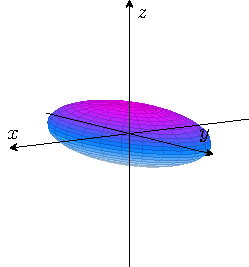
\includegraphics[scale=1]{./Images/quadric_surfaces/ellipsioid/ellipsioid.pdf}
	\caption{Illustration av en ellipsioid.}
	\label{fig:ellipsioid}
\end{figure}

\paragraph{Koner}
En kon beskrivs av en ekvation på formen
\begin{align*}
	\frac{x^2}{a^2} + \frac{y^2}{b^2} = \frac{z^2}{c^2}.
\end{align*}
\begin{figure}[!ht]
	\centering
	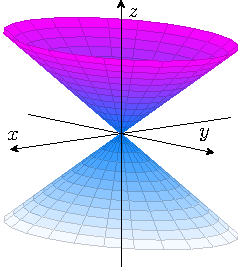
\includegraphics[scale=1]{./Images/quadric_surfaces/cone/cone.pdf}
	\caption{Illustration av en kon.}
	\label{fig:cone}
\end{figure}

\paragraph{Cylindrar}
En cylinder beskrivs av en ekvation på formen
\begin{align*}
	\frac{x^2}{a^2} + \frac{y^2}{b^2} = 1.
\end{align*}

\begin{figure}[!ht]
	\centering
	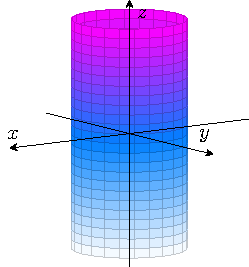
\includegraphics[scale=1]{./Images/quadric_surfaces/cylinder/cylinder.pdf}
	\caption{Illustration av en cylinder.}
	\label{fig:cylinder}
\end{figure}

\paragraph{Elliptiska paraboloider}
En elliptisk paraboloid beskrivs av en ekvation på formen
\begin{align*}
	\frac{x^2}{a^2} + \frac{y^2}{b^2} = \frac{z}{c}.
\end{align*}

\begin{figure}[!ht]
	\centering
	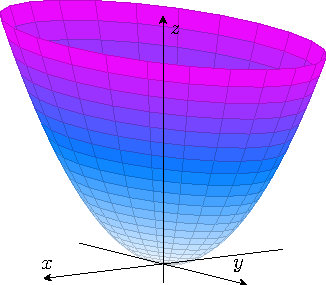
\includegraphics[scale=1]{./Images/quadric_surfaces/elliptic_paraboloid/elliptic_paraboloid.pdf}
	\caption{Illustration av en elliptisk paraboloid.}
	\label{fig:elliptic_paraboloid}
\end{figure}

\paragraph{Hyperbolska paraboloider}
En hyperbolsk paraboloid beskrivs av en ekvation på formen
\begin{align*}
	\frac{x^2}{a^2} - \frac{y^2}{b^2} = \frac{z}{c}.
\end{align*}

\begin{figure}[!ht]
	\centering
	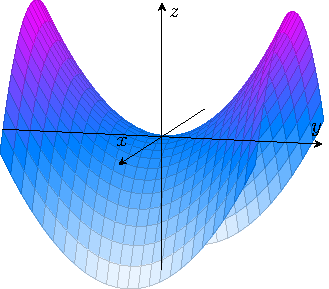
\includegraphics[scale=1]{./Images/quadric_surfaces/hyperbolic_paraboloid/hyperbolic_paraboloid.pdf}
	\caption{Illustration av en hyperbolsk paraboloid.}
	\label{fig:hyperbolic_paraboloid}
\end{figure}

\paragraph{Enmantlade hyperboloider}
En enmantlad hyperboloid beskrivs av en ekvationpå formen
\begin{align*}
	\frac{x^2}{a^2} + \frac{y^2}{b^2} - \frac{z^2}{c^2} = 1.
\end{align*}
\begin{figure}[!ht]
	\centering
	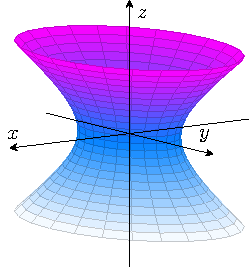
\includegraphics[scale=1]{./Images/quadric_surfaces/one_sheet_hyperboloid/one_sheet_hyperboloid.pdf}
	\caption{Illustration av en enmantlad hyperboloid.}
	\label{fig:one_sheet_hyperboloid}
\end{figure}

\paragraph{Tvåmantlade hyperboloider}
En tvåmantlad hyperboloid beskrivs av en ekvation på formen
\begin{align*}
	-\frac{x^2}{a^2} - \frac{y^2}{b^2} + \frac{z^2}{c^2} = 1.
\end{align*}

\begin{figure}[!ht]
	\centering
	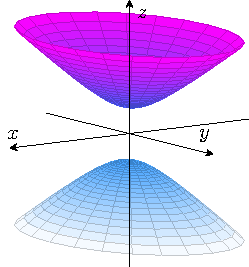
\includegraphics[scale=1]{./Images/quadric_surfaces/two_sheet_hyperboloid/two_sheet_hyperboloid.pdf}
	\caption{Illustration av en tvåmantlad hyperboloid.}
	\label{fig:two_sheet_hyperboloid}
\end{figure}

\section{Optimering}
Denna delen kommer handla om att försöka hitta minima till en funktion över ett rum. Att hitta maxpunkter är det samma som att byta tecken och hitta minimun, så vi fokuserar därför på att hitta minima.

\paragraph{Gyllene snitt-sökning}
Antag att $f$ är kontinuerlig och har endast ett lokalt minimum på $[a, b]$, och betrakta två punkter $x_{1}$ och $x_{2}$. Om $f(x_{1}) \leq f(x_{2})$ finns minimumspunkten på $[a, x_{2}]$, och om $f(x_{1}) \geq f(x_{2})$ finns minimumspunkten på $[x_{1}, b]$. Detta gäller eftersom derivatan endast byter tecken en gång på $[a, b]$, och vi med hjälp av funktionsvärdena i två punkter får information om derivatan imellan dessa punkterna. Man kan få en ganska säker metod vid att välja både $x_{1}$ och $x_{2}$ nära mitten av intervallet.

Metoden kan förbättras vid att återanvända funktionsvärden i kommande interationer. Sätt $a = b0, b = 1$. Vi väljer $x_{1}$ och $x_{2}$ symmetriskt och likformigt, så att $x_{2} = 1 - x_{1}$ och
\begin{align*}
	\frac{x_{1}}{x_{2}} = \frac{x_{2}}{1}.
\end{align*}
Vi kan lösa detta och få
\begin{align*}
	x_{1} = \frac{3 \pm \sqrt{5}}{2},\ x_{2} = \frac{\sqrt{5} - 1}{2}.
\end{align*}
Vi ser att $x_{2}$ är det gyllene snitt. Med detta val gäller att intervallängden avtar med en faktor $g$ per iteration.

\paragraph{Newtons metod}
Newtons metod för att hitta minima till en funktion $f(\vb{x})$ är att använda Newtons metod för att lösa ekvationssystemet $\grad{f}(\vb{x}) = \vb{0}$.

\paragraph{Gradientmetoden}
Vi vet att $f$ avtar snabbast i riktningen $-\grad{f}(\vb{x})$. Vi gör därför iterationen
\begin{align*}
	\vb{x}_{n + 1} = \vb{x}_{n} - \gamma_{n}\grad{f}(\vb{x}_{n}).
\end{align*}
$\gamma_{n}$ kan väljas konstant eller så att den minimerar $f(\vb{x}_{n + 1})$. Jämförd med Newtons

\section{Integration}

\paragraph{Eulers metod}
Antag att vi vill integrera en funktion $f$ över $[a, b]$. En enkel metod är att dela upp $[a, b]$ i $N$ steg, låta $x_{0} = a, x_{N} = b$. Eulers metod ger
\begin{align*}
	y_{N} &= y_{N - 1} + hf(x_{N - 1}) \\
	      &= y_{N - 2} + hf(x_{N - 2}) + hf(x_{N - 1}) \\
	      &\vdots \\
	      &= y_{0} + h\sum\limits_{i = 0}^{N - 1}f(x_{i}).
\end{align*}
Vi får slutligen approximationen
\begin{align*}
	\inteval{a}{b}{f(x)}{x} \approx h\sum\limits_{i = 0}^{N - 1}f(x_{i}).
\end{align*}

\subparagraph{Fel}
Utgå från differentialekvationen
\begin{align*}
	\dv{y}{x} = f, y(a) = y_{0},
\end{align*}
och antag att vi vill integrera $f$ över $[a, b]$. Analysens huvudsats ger
\begin{align*}
	\inteval{a}{b}{f(x)}{x} = y(b) - y(a).
\end{align*}
Att beräkna denna integralen är alltså helt ekvivalent med Eulers metod. Vi försöker därför först att hitta det lokala felet på $[x_{i}, x_{i + 1}]$, som enligt argumentet från Eulers metod ges av
\begin{align*}
	\abs{y_{i + 1} - y(x_{i + 1})} \leq \frac{1}{2}\abs{\deval[2]{y}{t}{c}}h^{2},
\end{align*}
där $c\in [x_{i}, x_{i + 1}]$. Enligt sats ges det globala felet då av
\begin{align*}
	\abs{y_{N} - y(x_{N})} \leq \frac{e^{L(a - b)}}{2L}\max\limits_{c\in [a, b]}\abs{\deval[2]{y}{t}{c}}h,
\end{align*}
där vi har ändrat derivatan för att vara säker på att den anger en övre begränsning av det lokala felet. Detta kan skrivas om till
\begin{align*}
	\abs{y_{N} - y(x_{N})} \leq \frac{e^{L(a - b)}}{2L}\max\limits_{c\in [a, b]}\abs{\deval{f}{t}{c}}h.
\end{align*}

\paragraph{Trapetsmetoden}
Betrakta integralen av en funktion $f$ över $[a, b]$. Dela nu upp $[a, b]$ i $N$ steg, och låt $x_{0} = a, x_{N} = b$. I trapetsmetoden interpolerar vi $f$ i $x_{i}$ och $x_{i + 1}$ och integrerar denna räta linjen. Integralen är lika med arean av en trapets, vilket vi enkelt kan beräkna. En approximation av integralen över $[x_{i}, x_{i + 1}]$ är därmed
\begin{align*}
	h\frac{f(x_{i + 1}) + f(x_{i})}{2}.
\end{align*}
En approximation av hela integralen är då
\begin{align*}
	\inteval{a}{b}{f(x)}{x} &\approx h\sum\limits_{i = 0}^{N - 1}\frac{f(x_{i + 1}) + f(x_{i})}{2} \\
	                        &= h\left(\frac{f(x_{0}) + f(x_{N})}{2} + \sum\limits_{i = 1}^{N - 1}f(x_{i})\right).
\end{align*}

\subparagraph{Fel}
Låt $T_{h}$ vara skattningsfelet av integralen med trapetsmetoden med steglängd $h$. Felet ges då av
\begin{align*}
	\abs{\inteval{a}{b}{f(x)}{x} - T_{h}} \leq \max\limits_{x\in [a, b]}\frac{1}{12}\abs{\deval[2]{f}{x}{x}}(b - a)h^{2}.
\end{align*}

För att visa detta, notera att det är ekvivalent att beräkna integralen av $f$ och att lösa begynnelsevärdesproblemet
\begin{align*}
	\dv{y}{x} = f(x),\ y(a) = y_{0}.
\end{align*}
Vi har en sats som beskriver det globala felet, och därmed behöver vi bara beräkna det lokala felet för integration mellan två punkter.

\paragraph{Simpsons metod}
Använder kvadratisk interpolation.

\subparagraph{Fel}
Låt $S_{h}$ vara skattningsfelet av integralen med Simpsons metod med steglängd $h$. Felet ges då av
\begin{align*}
	\abs{\inteval{a}{b}{f(x)}{x} - S_{h}} \leq \max\limits_{x\in [a, b]}\frac{1}{80}\abs{\deval[4]{f}{x}{x}}(b - a)h^{4}.
\end{align*}

\paragraph{Monte Carlo-integration}
Medelvärdesatsen för integraler ger att
\begin{align*}
	\frac{1}{b - a}\inteval{a}{b}{f(x)}{x} = f(c),
\end{align*}
där $f(c)$ är funktionens medelvärde på $[a, b]$. Vi kan skatta medelvärdet som
\begin{align*}
	\frac{1}{N}\sum\limits_{i = 1}{N}f(x_{i}),
\end{align*}
där alla $x_{i}$ är dragna oberoende från en likformig fördelning på $[a, b]$. Detta kallas för Monte Carlo-integration.

Metoden är helt analog i högre dimensioner.

\paragraph{Fel}
Om vi antar att alla $x_{i}$ dras från en likformig sannolikhetstäthet, kan vi skriva
\begin{align*}
	\frac{1}{b - a}\inteval{a}{b}{f(x)}{x} = \inteval{a}{b}{f(x)p(x)}{x},
\end{align*}
där $p$ är sannolikhetstätheten. Vänstersidan kan även skrivas som $\expec{f(X)}$.

Vi inför den stokastiska variabeln
\begin{align*}
	\varepsilon_{n} = \frac{1}{N}\sum\limits_{i = 1}{N}f(X_{i}) - \expec{f(X)}.
\end{align*}
Dens väntevärde ges av
\begin{align*}
	\expec{\varepsilon_{n}} &= \frac{1}{N}\sum\limits_{i = 1}{N}\expec{f(X_{i})} - \expec{f(X)} \\
	                         &= \expec{f(X)} - \expec{f(X)} \\
	                         &= 0.
\end{align*}
Vi har vidare
\begin{align*}
	\expec{\varepsilon_{n}^{2}} &= \expec{\left(\frac{1}{N}\sum\limits_{i = 1}^{N}f(X_{i}) - \expec{f(X)}\right)^{2}} \\
	                         &= \frac{1}{N^{2}}\expec{\left(\sum\limits_{i = 1}^{N}(f(X_{i}) - \expec{f(X)})\right)^{2}} \\
	                         &= \frac{1}{N^{2}}\expec{\left(\sum\limits_{i = 1}^{N}(f(X_{i}) - \expec{f(X)})\right)^{2}} \\
	                         &= \frac{1}{N^{2}}\expec{\left(\sum\limits_{i = 1}^{N}(f(X_{i}) - \expec{f(X)})\right)^{2}} \\
	                         &= \frac{1}{N^{2}}\expec{\sum\limits_{i = 1}^{N}(f(X_{i}) - \expec{f(X)})^{2} + \sum\limits_{n\neq m}(f(X_{n}) - \expec{f(X)})(f(X_{m}) - \expec{f(X)})} \\
	                         &= \frac{1}{N^{2}}\sum\limits_{i = 1}^{N}\expec{(f(X_{i}) - \expec{f(X)})^{2}} + \expec{\sum\limits_{n\neq m}(f(X_{n}) - \expec{f(X)})(f(X_{m}) - \expec{f(X)})} \\
	                         &= \frac{\sigma_{f}^{2}}{N} + 0.
\end{align*}
Korstermerna har väntevärde
\begin{align*}
	\expec{(f(X_{n}) - \expec{f(X)})(f(X_{m}) - \expec{f(X)})} &= \expec{f(X_{n}) - \expec{f(X)}}\expec{f(X_{m}) - \expec{f(X)}} \\
	                                                           &= 0,
\end{align*}
då de olika $X_{i}$ är oberoende. Därmed är standardavvikelsen av $\varepsilon_{N}$ lika med $\frac{\sigma}{\sqrt{N}}$, och felet i metoden är proportionellt mot $\frac{1}{\sqrt{N}}$.

Vi noterar att centrala gränsvärdesatsen ger att $\nu = \frac{\sqrt{N}}{\sigma}\varepsilon_{N}$ är standard normalfördelat.

I $d$ dimensioner är felet proportionellt mot $N^{-\frac{d}{2}}$, och vi ser att den är bättre än trapetsmetoden för $d > 4$.

\section{Ytor}

\subsection{Definitioner}

\paragraph{Ytor}
En yta är en funktion $\vect{r}: D\to\R^3$ med $D\subset\R^2$.

\paragraph{Tangentplan}
Tangentplanet till en kurva spänns upp av vektorerna
\begin{align*}
	\vect{r}_s(s, t) = \left(\deval{r_1}{s}{s, t}, \deval{r_2}{s}{s, t}, \deval{r_3}{s}{s, t}\right), \\
	\vect{r}_t(s, t) = \left(\deval{r_1}{t}{s, t}, \deval{r_2}{t}{s, t}, \deval{r_3}{t}{s, t}\right), \\.
\end{align*}

\paragraph{Positiv sida av yta}
Den positiva sidan av en yta är den sidan nromalvektorn $\pdv{\vect{r}}{s}\times\pdv{\vect{r}}{t}$ pekar mot.

\paragraph{Enhetsnormal}
\begin{align*}
	\vect{N} = \frac{\pdv{\vect{r}}{s}\times\pdv{\vect{r}}{t}}{\abs{\pdv{\vect{r}}{s}\times\pdv{\vect{r}}{t}}} 
\end{align*}
är en ytas enhetsnormal.

\paragraph{Areaelement}
\begin{align*}
	\dd{S} = \abs{\pdv{\vect{r}}{s}\times\pdv{\vect{r}}{t}}\dd{s}\dd{t}
\end{align*}
ör en ytas arealement.

\paragraph{Vektoriellt arealement}
\begin{align*}
	\dd{\vect{S}} = \vect{N}\dd{S} = \pdv{\vect{r}}{s}\times\pdv{\vect{r}}{t}\dd{s}\dd{t}
\end{align*}
är ytans vektoriella areaelement.

\paragraph{Area av yta}
Låt $\vect{r}: D\to\R^3$ vara en parametrisering av en yta $Y$. Då ges arean av
\begin{align*}
	A_Y = \inteval{D}{\abs{\pdv{\vect{r}}{s}\times\pdv{\vect{r}}{t}}}{{s, t}}. 
\end{align*}
Detta skrivs även
\begin{align*}
	A_Y = \iint_{Y}\dd{S}.
\end{align*}

\paragraph{Integration av skalärfunktioner över ytor}
Låt $\vect{r}: D\to\R^3$ vara en parametrisering av en yta $Y$. Då ges integralet av funktionen $f$ över $Y$ av
\begin{align*}
	\inteval{D}{f(\vect{r}(s, t))\abs{\pdv{\vect{r}}{s}\times\pdv{\vect{r}}{t}}}{{s, t}}
\end{align*}
och betecknas
\begin{align*}
	\iint\limits_{Y}f(\vect{r})\dd{S}.
\end{align*}

\paragraph{Flöde genom yta}
\begin{align*}
	\fint{Y}{\vect{u}}{\vect{S}}
\end{align*}
ör flödet av $\vect{u}$ genom $Y$.

\subsection{Satser}

\section{Samband mellan integraler}

\paragraph{Greens sats}
Låt
\begin{itemize}
	\item $\Omega\subset\R^2$ vara öppen.
	\item $P, Q: \Omega\to\R$ är $C^1$.
	\item $D\subset\Omega$ är kompakt.
	\item $\bound{D}$ vara styckvis $C^1$.
\end{itemize}

Då gäller att
\begin{align*}
	\oint\limits_{\bound{D}}P\dd{x} + Q\dd{y} = \inteval{D}{\pdv{Q}{x} - \pdv{P}{y}}{{x, y}}.
\end{align*}
Märk att det första integralet kan skrivas som ett kurvintegral av ett vektorfält.

\proof
Beviset ges enbart för en rektangel. Det allmäna beviset involverar att betrakta flera små rektanglar.

\begin{align*}
	\inteval{D}{\pdv{Q}{x} - \pdv{P}{y}}{{x, y}} &= \int\limits_{c}^{d}\int\limits_{a}^{b}\pdv{Q}{x}(x, y)\dd{x}\dd{y} - \int\limits_{a}^{b}\int\limits_{c}^{d}\pdv{P}{y}(x, y)\dd{y}\dd{x} \\
	                                           &= \int\limits_{c}^{d}Q(b, y) - Q(a, y)\dd{y} - \int\limits_{a}^{b}P(x, d) - P(x, c)\dd{x}.
\end{align*}

Dela randen till rektangeln upp i $\gamma_1, \gamma_2, \gamma_3, \gamma_4$, där dessa beskrivas av $x = b, y = d, x = a, y = c$ respektiva. Då kan det sista integralet skrivas som
\begin{align*}
	  \int\limits_{\gamma_1}Q(x, y)\dd{y} + \int\limits_{\gamma_2}P(x, y)\dd{x} + \int\limits_{\gamma_3}Q(x, y)\dd{y} + \int\limits_{\gamma_4}P(x, y)\dd{x}.
\end{align*}	  
Varje integral över randen involverar enbart en variabel och en funktion. Därmed kan vi lägga till integralet över den andra variabeln av den andra funktionen och få
\begin{align*}
	\left(\int\limits_{\gamma_1} + \int\limits_{\gamma_2} + \int\limits_{\gamma_3} + \int\limits_{\gamma_4}\right)P(x, y)\dd{x} + Q(x, y)\dd{y} = \int\limits_{\bound{D}}P(x, y)\dd{x} + Q(x, y)\dd{y},
\end{align*}
och beviset är klart.

\paragraph{Divergenssatsen}
Låt $\vect{u}$ vara ett $C^1$-vektorfält definierat i en öppen mängd $\Omega\subset\R^3$, $K\subset\Omega$ vara kompakt och $\bound{K}$ bestå av en eller flera $C^1$-ytor med utadriktad normal. Då gäller att
\begin{align*}
	\fint{\bound{K}}{\vect{u}}{\vect{S}} = \inteval{K}{\div{\vect{u}}}{{x, y, z}}.
\end{align*}

\proof
Beviset ges enbart för ett rätblock. Det allmäna beviset involverar att betrakta flera rätblock, tror jag.

Vi delar integralerna upp som
\begin{align*}
	&\fint{\bound{K}}{\vect{u}}{\vect{S}} = \sum\limits_{i}\fint{\bound{K}}{u_i\vect{e}_i}{\vect{S}}, \\
	&\inteval{K}{\div{\vect{u}}}{{x, y, z}} = \sum\limits_{i}\inteval{K}{\div{u_i\vect{e}_i}}{{x, y, z}}
\end{align*}
och ser att det räcker att visa att
\begin{align*}
	\fint{\bound{K}}{u_i\vect{e}_i}{\vect{S}} = \inteval{K}{\div{u_i\vect{e}_i}}{{x, y, z}}, i = 1, 2, 3.
\end{align*}
I fallet $i = 1$ får man
\begin{align*}
	\fint{\bound{K}}{u_i\vect{e}_i}{\vect{S}} &= \int\limits_{e}^{f}\int\limits_{c}^{d}u_1(b, y, z)\dd{y}\dd{z} - \int\limits_{e}^{f}\int\limits_{c}^{d}u_1(a, y, z)\dd{y}\dd{z} \\
	                                          &= \int\limits_{e}^{f}\int\limits_{c}^{d}\int\limits_{a}^{b}\pdeval{u_1}{x}{x, y, z}\dd{x}\dd{y}\dd{z}\\
	                                          &= \int\limits_{e}^{f}\int\limits_{c}^{d}\int\limits_{a}^{b}\div{u_i\vect{e}_i}\dd{x}\dd{y}\dd{z}.
\end{align*}

Med ett motsvarande bevis för $i = 2, 3$ är beviset klart.

\end{document}
